\begin{framedpage}{theorem}{Five Color Theorem}{ 
    Every planar graph is 5 colorable. \label{emb:thm:5color}}

    Again, we prove by induction on removing a small degree vertex. Let $G$ be a graph, and pick a vertex $v$ of degree 5. By our induction hypothesis, we can come up with a $5$-coloring of the graph $G\setminus v$. We may assume that the neighborhood of $v$ sees all 5 colors, otherwise we would be done. As such, index $N(v)$ by colors $\{v_1, v_2, v_3, v_4, v_4\}$. Furthermore, as we are in a planar graph, we may take this labeling to proceed cyclically around $v$. We now use a trick very similar to the proof of \ref{thm:brooks}. \\
   For each $i$ and $j$, let $H_{ij}$ be the $ij$ colored subgraph of $G\setminus v$. Then either $v_i$ and $v_j$ belong to the same connected component of $H_{ij}$, or not. In the case they do not, we can switch the colors $i, j$ in the connected component containing $v_i$, and now the neighborhood of $v$ only has 4 colors. \\
   Suppose instead that for each $i, j$, the vertices $v_i$ and $v_j$ belong to the same connected component. This means that there is a path $P_{1,3}$ from $v_1$ to $v_3$, which is only colored with colors $1, 3$.\\
    Similarly, there must be a path $P_{2, 4}$ from $v_2$ to $v_4$ which is only colored with vertices colored $2$ and $4$. As these paths get different colors, we know that they are disjoint from each other. 
    \begin{itemize}
     \item Suppose there is not an $i,j$ colored path between $v_i$ and $v_j$ . Then $v_i$ and $v_j$ belong to separate connected components of the subgraph colored $i,j$, therefore in one component we can switch their colors, This reduces the colors in the neighborhood of $v$ to 4 colors, so we can color the graph with 5 colors. 
     \item The above must be the case, as a 13 path cannot intersect a 24 path, but the existence such paths would create a topological $K_{3,3}$ within our graph, contradicting planarity.
     \[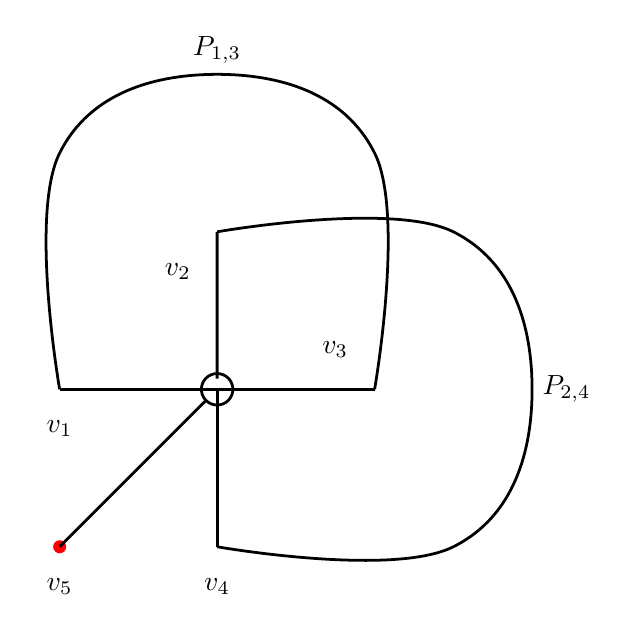
\begin{tikzpicture}

   \newcommand{\vertexradius}{2.5pt}
\newcommand{\vertexscale}{.5}
\newcommand{\bigvertexscale}{2}
\newcommand{\vertex}{\node[circle, fill=black, scale=\vertexscale] }
\newcommand{\vertexa}{\node[circle, fill=red, scale=\vertexscale] }
\newcommand{\highlighta}{red!20}
\newcommand{\highlightb}{blue!20}
\newcommand{\highlightc}{green!20}
\newcommand{\shadinga}{gray!20}
\newcommand{\smallvertex}{\node[circle, fill=black, scale=.2]}
\newcommand{\highlightlinewidth}{3pt}

\tikzset{every path/.style={line width=1 pt}}
   \vertexc at (0,1) {};
   \vertexa at (-2,-3) {};
   \vertexd at (0,-3) {};
   \vertexb at (-2,-1) {};
   \vertexe at (2,-1) {};
   \draw[fill=white] (0,-1) node (v1) {} circle[radius=.2];
   \draw (-2,-3) -- (v1) -- (0,1);
   \draw (-2,-1) -- (0,-1) -- (0,-3);
   \draw (2,-1) -- (0,-1);
   \node at (-2,-1.5) {$v_1$};
   \node at (-0.5,0.5) {$v_2$};
   \node at (1.5,-0.5) {$v_3$};
   \node at (0,-3.5) {$v_4$};
   \node at (-2,-3.5) {$v_5$};
   \draw  plot[smooth, tension=.7] coordinates {(-2,-1) (-2,2) (0,3) (2,2) (2,-1)};
   \draw  plot[smooth, tension=.7] coordinates {(0,1) (3,1) (4,-1) (3,-3) (0,-3)};
   
   \vertexc at (3,-3) {};
   \vertexd at (3,1) {};
   \vertexb at (2,2) {};
   \vertexe at (-2,2) {};
   \node[above] at (0,3) {$P_{1,3}$};
   \node[right] at (4,-1) {$P_{2,4}$};
   \end{tikzpicture}\] 
    \end{itemize}
\end{framedpage}